\documentclass{article}

\usepackage[utf8]{inputenc}
\usepackage{graphicx}		% Graphics.
\usepackage{color}
\usepackage[english]{babel}
\usepackage{float}
\usepackage{subcaption}
\usepackage{xfrac}
\usepackage{matlab-prettifier}
\usepackage{amsmath}    
\usepackage{amssymb}
\usepackage{siunitx}
\usepackage{chemformula}
\usepackage{physics}
\usepackage{pdfpages}
\usepackage{wrapfig}
\usepackage[justification=centering]{caption}

% Create a separate table for the appendix.
\usepackage[toc,page]{appendix}

% Table of Content has fast links to sections.
\usepackage{hyperref}

% Remove dots in table of contents.
\usepackage[titles]{tocloft}
\renewcommand{\cftdot}{}

% Page style.
\usepackage[top=2cm, bottom=2cm, left = 2cm, right = 2cm]{geometry}
\setlength{\parindent}{0pt}	% Disable indents.

% BIBTEX.
\usepackage[style=ieee]{biblatex}
\usepackage{csquotes}
\addbibresource{references.bib}

\begin{document}

%----------------------------------------------------------------------------------------
%	Title page.
%----------------------------------------------------------------------------------------
\input{chapters/titlepage.tex}


%----------------------------------------------------------------------------------------
%	TABLE OF CONTENT.
%----------------------------------------------------------------------------------------
\newpage				% Start at new page.
\pagenumbering{arabic}	% Page numbering reset & style.
\renewcommand{\contentsname}{Table of Contents}
\tableofcontents		% Add table of content.


%----------------------------------------------------------------------------------------
%	INTRODUCTION (1).
%----------------------------------------------------------------------------------------
\newpage
%----------------------------------------------------------------------------------------
%	INTRODUCTION.
%----------------------------------------------------------------------------------------
%example MISC \cite{exampleMISC}.\\
%example Book \cite{exampleBOOK}.\\
%example article \cite[p.~5]{exampleARTICLE}

\section{Introduction}
The purpose of this report is to relate space weather events with analyzed data from EISCAT.
The end result of this practical is to become acquainted with data from EISCAT and the programs used to analyze it.
This report will be analyzing data from the EISCAT radar through the use of GUISDAP. 
The pre-analyzed data comes from EISCAT through Madrigal database.
With GUISDAP and Madrigal, the plots will be interpreted to find relationships with space weather. 

\subsection{Space Weather}
The effect from the sun and the other extraplanetary sources on the Earth is called space weather. 
The influence of space weather on Earth include the aurora, disturbances in magnetosphere and ionosphere, and geomagnetic induced currents \cite{I_NOAA_2}. 
The causes of the space weather originates from the sun which includes coronal mass ejections, solar flares, and coronal holes.
There are several effects originating from space weather: damaging spacecraft electronics, increased drag affecting orbit of satellites, increasing radiation dosage in astronauts and airplane passengers, causing radio blackouts on Earth, and causing electrical power grid power outages.
Space weather can be observed by ground-based systems or by satellites. Ground-based systems involve telescopes observing the photosphere, neutron detectors, and measuring the ionosphere.
Many current satellites carry sun monitoring sensors as secondary payloads.
There are mathematical models that can simulate the space weather environment.

\subsection{Solar Storms of Halloween 2003}
The space weather event  occurred between October 19$^{th}$ and November 7$^{th}$ and is referred to as the Halloween solar storms. 
It occurred during the later part of solar cycle 23. It was not expected during the quieter part of the solar cycle.
It had a large affect on Earth, with aurora seen in Florida, satellites and communications being affected, and a power outage is Sweden lasting for a hour \cite{I_NASA_1}. 
It was composed of 17 flares ranging in strength, with the largest being estimated at X28 power causing a R5 radio blackout and numerous anomalies in satellites. 
This space weather event included the 4$^{th}$ largest flare in recorded history \cite{I_NOAA}.



%----------------------------------------------------------------------------------------
%	GUISDAP (3).
%----------------------------------------------------------------------------------------
\newpage
%----------------------------------------------------------------------------------------
%	GUISDAP.
%----------------------------------------------------------------------------------------

\section{GUISDAP software}
In this section the raw EISCAT data is processed using the MATLAB software with the package GUISDAP. The data analyzed in this section was obtained with the 42m radar located in Svalbard, Norway. The time frame of the analyzed data corresponds to the 27th of October, 2016, from 15:00 to 21:00.
\newline
\newline
GUISDAP have several "experiment" methods. From the EISCAT experiments manual: "An EISCAT experiment is a set of instructions telling the transmitters, receivers and digital signal processing units what to do at what time". Meaning that depending on the object of interest of the experimenter, Some of the parameters that change between experiments are the code length in bits, baud length, smapling rate, the range span (measurable height), time resolution, etc. In this particular case, the experiment "ipy" was used. 
%\begin{tabular}[H]{c | c}
%	Version & 4.2 \\\hline
%	Antenna & Single, switchable\\\hline
%	
%\end{tabular}
\newline
\newline
With the help of GUISDAP, a few plots showing different parameters observed in the ionosphere at the time period mentioned above. The following parameters are used by the ipy experiment. One of the obtained parameters is the raw electron data. The data obtained with GUISDAP which is data measured from the EISCAT radar, was compared with data formulated using the IRI model in the following pictures.

\begin{minipage}{0.45\textwidth}	
	\begin{flushleft}
	\begin{figure}[H]
		\centering
		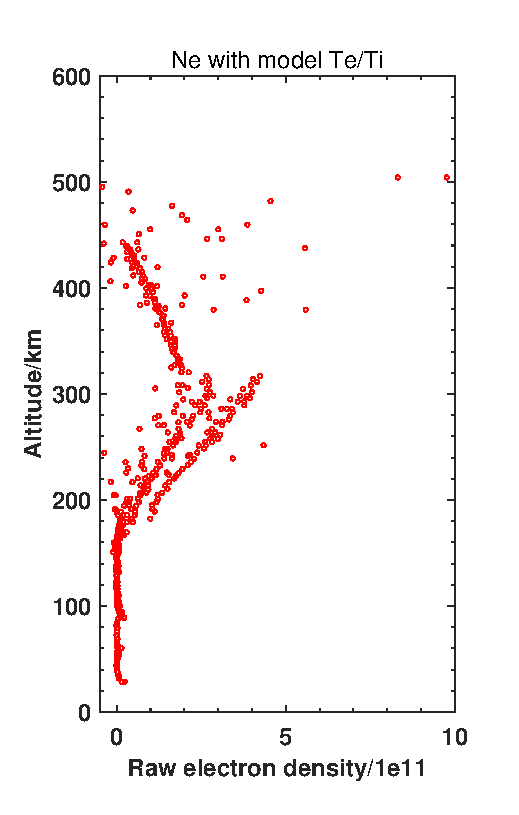
\includegraphics[width=\textwidth]{figures/rawNe.eps}
		\caption{Electron density data obtained from EISCAT 2016-10-27.}
		\label{fig::NeE}
	\end{figure}
	\end{flushleft}
\end{minipage}
\begin{minipage}{0.45\textwidth}
	\begin{flushright}
	\begin{figure}[H]
	\centering
	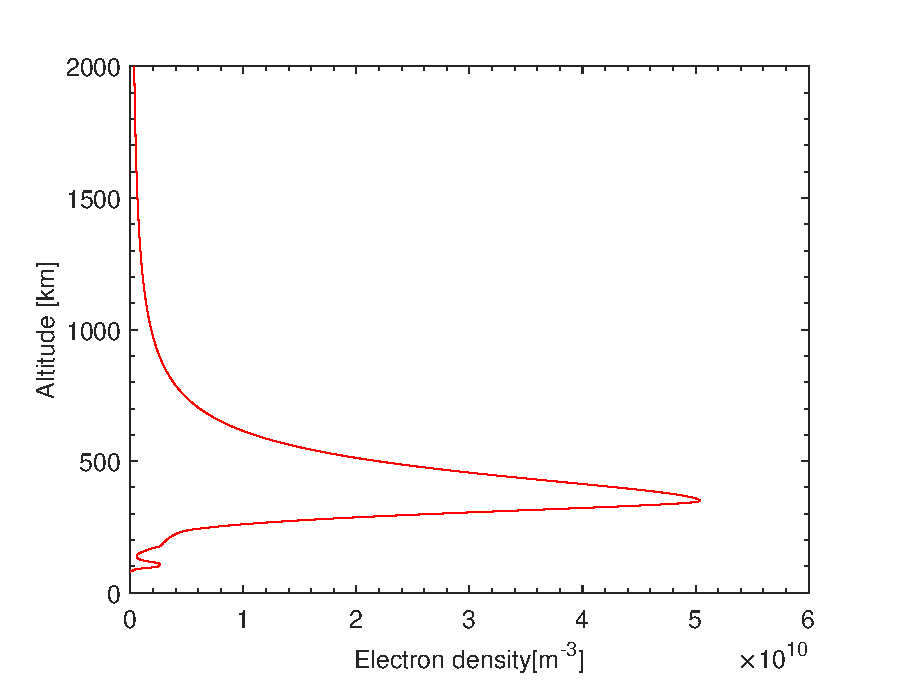
\includegraphics[width=\textwidth]{figures/NeIRI.eps}
	\caption{Electron density data from the IRI model 2016-10-27}
	\label{fig::NeIRI1}
	\end{figure}
	\end{flushright}
\end{minipage}

In these two images, the electron density from 0 to 600 km was plotted in order to compare the IRI model to the measurements from EISCAT. Both are showing the electron density distribution at around 18:00 hours. While both the model and measurements agree on where the maximum occurs, the model underestimates the amount of electrons by about a factor of 3. This discrepancies can be attributed to any assumptions that the model might take.

\begin{figure}[H]
	\centering
	\includegraphics[width=0.90\textwidth]{figures/Results.eps}
	\caption{Plot produced analyzing raw data from EISCAT with GUISDAP}
	\label{fig::resultsE1}
\end{figure}

Figure \ref{fig::resultsE1} shows the results of analyzing 6 hours of data obtained by EISCAT from 15:00  to 21:00 on the 27th of October 2016. In the first row, we can see the electron density which matches with the plots on figure \ref{fig::NeE} and figure \ref{fig::NeIRI1}, showing a maximum around 300 km of altitude. The second row shows the electron temperature, with respect to each altitude, it is interesting to note that most of the times the variation is smooth and small, except for a small band right before 18:00 and a larger band around 20:30. The third row row shows the ion temperature, again, this one is more or less constant along time with a few exceptions around 17:30 and 18:00. The fourth row showing the ion drift velocity,  most of the values look like a more or less random noise, meaning that this drift velocity is not consistent. On the fifth and final row we see the data of the antenna  within the time range of the data analyzed.


%----------------------------------------------------------------------------------------
%	SPACEWEATHER EVENT (3).
%----------------------------------------------------------------------------------------
\newpage
%----------------------------------------------------------------------------------------
%	SPACEWEATHER EVENT.
%----------------------------------------------------------------------------------------
\section{Space weather event}
\begin{wrapfigure}[18]{r}{6cm}
\includegraphics[width=6cm]{figures/SW_aurora_29oct_3.jpg}

\caption{Geomagnetic storm/ Aurora on the 29th of October \cite{spaceweather}.}
\label{fig:Aurora3}
\end{wrapfigure} 
In the rest of this document preprocessed data is used from the Halloween 2003 space weather event. This event took place from the 28th up to the 29th of October, with the main two peaks at 11:10 (28-10-2003) and 20:50 (29-10-2003) \cite{goes_x-ray_archive}. This solar weather event consisted of a series of solar flares and coronal mass ejections. The solar flare with the most energy was measured at 10:16:53 UCT. With an energy of $6.9\cdot10^{25}$\,Joule and a mass of $1.6 \cdot 10^{10}$\,gram \cite{CME_list}, one of the strongest ever measured by GOES.\\

Satellite-based systems and communications were affected, as well as the instruments onboard \cite{swpc-noaa}. Aircraft were advised to avoid high altitudes near the polar regions, and a one-hour-long power outage occurred in Sweden as a result of the solar activity. Auroras (figure \ref{fig:Aurora3}) were observed at latitudes as far south as Texas and the Mediterranean countries of Europe \cite{wiki_halloween_solar_stroms}.

\subsection{Solar flares}
\begin{wrapfigure}[15]{r}{0.5\textwidth}
\includegraphics[width=.5\textwidth]{figures/SW_CME.jpg}

\caption{Solar image of a CME using a cronagraph\cite{spaceweather}.}
\label{fig:SW:CME}
\end{wrapfigure} 

On the 28th 12:18 UCT one of the most powerful Coronal Mass Ejections (CME) in years erupted, this eruption, that caused a intense geomagnetic storm, is shown in figure \ref{fig:SW:CME}.The solar flares erupted out of 486 giant sunspots. It was measured X17  on the Richter scale of solar flares. This means that the peak had an energy above $7 \cdot 10^{-4}$\,W/m$^2$. It was also classified as a S3 storm, which means it has a flux of more than $10^3$ with $\geq$10\,MeV particles.  \cite{spaceweather}.\\


%----------------------------------------------------------------------------------------
%	GOES.
%----------------------------------------------------------------------------------------
\subsection{GOES}
In figure \ref{fig:goes_sem_data_oct} the space weather data from GOES10 (10th Geostationary Operational Environmental Satellite) over the month October is shown. In figure \ref{fig:goes_sem_data_nov} the data from the same satellite is shown over the month of November \cite{ngdc-noaa}. \\

In the top plot the peak flux of the solar flares/ CMEs in watts per square meter (W/m$^2$) between 1 and 8 Ångströms. Based on the flux the solar flare is classified. These are the classifications:
\begin{enumerate}
	\item Class A: flux $< 10^{-7}$
	\item Class B: $10^{-7} \leq$ flux $< 0^{-6}$
	\item Class C: $10^{-6} \leq$ flux $< 0^{-5}$
	\item Class M: $10^{-5} \leq$ flux $< 0^{-4}$
	\item Class X: flux $\geq 10^{-4}$
\end{enumerate}

In the second top plot the electrons flux, directed to Earth, is shown in e$^{-}$cm$^{-}2$s$^{-1}$sr$^{-1}$. With the black line presenting electrons with an energy greater than 0.6\,MeV, red above 2\,MeV and green above 4\,MeV. In the third plot the proton flux is shown, with the energies greater than 1\,MeV for black, 5\,MeV for red, 10\,MeV for green, 30\,MeV for pink, 50\,MeV for blue, 60\,MeV purple and 100\,MeV for light blue. In the last plot the magnetic field strength in nT, where black (Hp) is the magnetic field vector component, points northward, perpendicular to the orbit plane which for a zero degree inclination orbit is parallel to Earth's spin axis. Red (He) is the magnetic field vector component, perpendicular to Hp and Hn and points earthward. Green (Hn) is the magnetic field vector component, perpendicular to Hp and He and points eastward. \\


\begin{figure}[H]
\centering
\includegraphics[page=1, width=.79\textwidth]{figures/goes10_oct.pdf}

\caption{GOES10 data from the month October 2003 \cite{ngdc-noaa}.}
\label{fig:goes_sem_data_oct}
\end{figure}

\begin{figure}[H]
\centering
\includegraphics[page=1, width=.79\textwidth]{figures/goes10_nov.pdf}

\caption{GOES10 data from the month November 2003 \cite{ngdc-noaa}.}
\label{fig:goes_sem_data_nov}
\end{figure}

From the GOES data in figure \ref{fig:goes_sem_data_oct} and \ref{fig:goes_sem_data_nov} it can clearly be seen that the were a lot of instabilities during the end of October and the beginning of November. Starting around the 14th of October the magnetic field became more instable and the proton flux increased. On the 18th the electron flux increased, as well as the flux of energy. The main two peaks where at the 28th and 29th of October, followed by some less, but still pretty strong, flares on the 2nd, 3rd and 4th of November. After the sixth of November the fluxes went down again.


%----------------------------------------------------------------------------------------
%	IMAGE.
%----------------------------------------------------------------------------------------
\subsection{IMAGE}

In figure \ref{fig:image_grams} the magnetometer data from multiple latitudes on Earth from the 29th of October to the 1st of November is shown. These values differ from the magnetometer data from GOES due to that GOES is orbiting Earth and these magnetometers are located on a fixed position on the Earth. It can be seen that the latitudes around the Auroral oval have the largest spikes. 

\begin{figure}[H]
        \begin{subfigure}[b]{0.33\textwidth}
                \includegraphics[width=\linewidth]{figures/IMAGE_X_gram.jpg}
                \caption{Perpendicular to the Y and Z axis (Hn) \cite{image}.}
				\label{fig:image_x_gram}
        \end{subfigure}%
        \begin{subfigure}[b]{0.33\textwidth}
                \includegraphics[width=\linewidth]{figures/IMAGE_Y_gram.jpg}
                \caption{Perpendicular to the z axis, pointing Eastward (He) \cite{image}.}
				\label{fig:image_y_gram}
        \end{subfigure}%
        \begin{subfigure}[b]{0.33\textwidth}
                \includegraphics[width=\linewidth]{figures/IMAGE_Z_gram.jpg}
                \caption{Axis from the center of the Earth northwards (Hp)\cite{image}.}
				\label{fig:image_z_gram}
        \end{subfigure}
        \caption{Magnetogram data from IMAGE (International Monitor for Auroral Geomagnetic Effects).}
        \label{fig:image_grams}
\end{figure}






%----------------------------------------------------------------------------------------
%	EISCAT MADRIGAL (2).
%----------------------------------------------------------------------------------------
%\newpage
%----------------------------------------------------------------------------------------
%	EISCAT MADRIGAL.
%----------------------------------------------------------------------------------------

\section{EISCAT Madrigal}
In figure \ref{fig:madrigal} the EISCAT data from the 30th of October 2003 is shown. There are a few white gaps which can be explained by interference like clouds in the atmosphere. On top we have the electron density, followed by the electron temperature, ion temperature, ion drift velocity and the system temperature. \\

Around 20:50 on the 29th of October 2003, one of the main peaks during this solar storm was measured. When this peak was over there was a dip in electron density, as can be seen from figure \ref{fig:madrigal}. Then, on the 30th of October there were some M-flares at 1:55 till 2:45 and 15:20 till 15:40 measured by GOES \cite{goes_x-ray_archive}. You can see in the EISCAT data that right after this change has been measured the densities and temperatures started increasing. The peaks are delayed by a a couple of hours in this data. \\

When comparing the data from the 30th of October 2003 to a more quit day, like the one in figure \ref{fig::resultsE1}, it can be seen that especially the fluctuations are way more intense. The gradient between upper and lower in the atmosphere is still present. But everything is, on average, more intense. The perturbations go deeper into the atmosphere and with higher velocities.





\begin{figure}
\centering
\includegraphics[width=.9\textwidth]{figures/2003-10-30_SvalvardPlot.png}
\caption{EISCAT radar data from the upper atmosphere science database Madrigal \cite{madrigal}.}
\label{fig:madrigal}
\end{figure}


%----------------------------------------------------------------------------------------
%	INTER-NATIONAL REFERENCE IONOSPHERE (IRI) MODEL (1-2).
%----------------------------------------------------------------------------------------
\newpage
\input{chapters/iri-model.tex}


%----------------------------------------------------------------------------------------
%	DISCUSSION MADRIGAL AND IRI MODEL (1).
%----------------------------------------------------------------------------------------
\newpage
%----------------------------------------------------------------------------------------
%	DISCUSSION.
%----------------------------------------------------------------------------------------

\section{Discussion}
%example MISC \cite{exampleMISC}.\\
%example Book \cite{exampleBOOK}.\\
%example article \cite[p.~5]{exampleARTICLE}

The effects of solar flares are easily observed in Figure \ref{fig:madrigal}.
There is a strong increase in the electron density, a decrease in electron temperature, fluctuations in the ion temperatures, and changes in ion drift values.
Handzo \cite{Handzo} looked at X-class flares effects in the atmosphere and saw strongly increased electron density peaking after the the flare and the perturbation lasting a long time. This large difference between the actual electron density and the IRI-model estimate is shown in Figure \ref{fig::IRIvsMa}. The electron density during the storm is approximately a magnitude larger than the approximated model. The disturbance peaked after the solar flare and lasted for approximately an hour afterwards. After this time period, the electron density suddenly enters a depleted state with a lower electron density than prior to the flare.
The electron temperature is shown as decreased during and after the solar flare. This is contrary to the accepted notion of highest electron temperatures during the strongest solar storms \cite{Caspi}. This discrepancy between the the data shown and the expected results of the higher temperatures could be explained with differentiated plasma. This concept is explained in Battaglia \cite{Battaglia}, where there is cool core and the heated outer regions. Battaglia mentioned this could also be due to the cooler plasma in the foreground interacting with the higher temperature plasma.
During a solar flare, the ion temperatures can fluctuate during the solar storm due to positive and negative effects \cite{ITemp}. The ion temperature and the ion density interact interact causing an unpredictable variations. The temperature for the case of this Halloween storm fluctuated but remained higher than normal.
The solar flare has a positive and negative effect on $E \times B$ ion drift velocities \cite{IDrift}. There is a short lasting severe decrease in velocities and a longer lasting, much weaker increase in ion velocities.


%----------------------------------------------------------------------------------------
%	CONFIRMATION OF PARTICIPATION (1).
%----------------------------------------------------------------------------------------
\section{Confirmation of Participation}
Hereby, A. Hoehne, D. Talavera and E.F.M. Weterings declare to have participated and collaborated in this report.


%----------------------------------------------------------------------------------------
%	REFERENCES (1).
%----------------------------------------------------------------------------------------
\newpage				% Start at new page.
\addcontentsline{toc}{section}{References}
\printbibliography



\end{document}
